\chapter{Experiments and Results}
\section{Implementation}
We performed all of our experiments within Google's Tensorflow \cite{abadi2016tensorflow} framework.
Tensorflow imposes a style of computation which is not immediately adaptable to our experiments, but it was nevertheless chosen for its prevalence and impact on current methods.
Its popularity has largely affected the number of open-source code samples available, and many current architectures have clear examples in Tensorflow.
The thriving ecosystem of open-source contributions around Tensorflow proved to be a highly beneficial factor in providing a variety of existing architectures for experimentation.

As was noted before, Tensorflow operates in a slightly different way than many other libraries.
Rather than allowing the user to chain together operations at random, it fixes a computational graph which defines the full model.
Google's developers preferred this static model as it is generally well-suited to a lot of deep learning research, while also being flexible enough to allow distributed computing (of crucial importance to a a cloud company like Google).
This, however, poses an obvious problem with our algorithm, which is largely dynamic.
A few workarounds had to be developed in order to interface with the static computational graph.
While it is possible to use conditional blocks to disable parts of the graph, it is impossible to insert during runtime.
As such, the entire possible network capacity has to be allocated upfront, which potentially reduces the range of experimentation.
This additionally means that while parts of the network can be disabled, they still take important parameter space which cannot be reallocated to other parts of the network.

In his work on spatially-sparse convolutional neural networks \cite{graham2014spatially}, Graham noted that there are potential improvements in architecture by performing sparse convolutions.
Tensorflow does not support such functionality at the moment, although it appears that they may be planning its development for the future \cite{spatiallysparseconv}.
For our experiments, we continue to rely on densely-connected convolutional layers for the
% EXPLAIN PLS

Other libraries were explored briefly, but they either did not provide the necessary flexibility or have a reasonable set of tutorials/examples to facilitate the work here.
For example, one of the more common tools in imag e-based deep learning has been Caffe \cite{jia2014caffe}, which boasts well-tuned performance as well as a public repository of models in the Caffe Model Zoo.
Unfortunately, being written almost entirely in C++, it is largely unamenable to testing and infrastructure development.
Modifying Caffe to implement new training methods typically requires a significant contribution in C++, which requires an overhead not often undertaken except by researchers with significant prior experience.
Furthermore, models are loaded in a fixed format, which hampers the ability to dynamically redefine networks.
On the other side of the spectrum are libraries like Keras, which usually serve as a higher-level wrapper to other deep learning libraries.
They were generally judged as being insufficiently expressive for the type of modifications we performed, so we considered other options.

All experimentation was performed on a GTX 1060, which was provided via a grant from Princeton SEAS.
GPU computation has widely become the standard for deep learning computation in recent years, as it can provide nearly an order of magnitude in performance.
Particularly for models like modern residual networks, which can take days to converge to reasonable accuracy, it is nearly impossible to train neural networks on CPU servers.
Tensorflow still utilizes the CPU extensively to coordinate training and perform a significant amount of calculations, but modern-day GPUs are nearly perfectly designed for the type of computations required for convolutions.

A recent glut of libraries aimed at helping automate the deep learning deployment process has led to a variety of different methods.
NVIDIA's CUDA and CUDNN libraries, both of which re crucial for the performance of modern deep learning libraries, require a complex set of dependencies and installation procedures.
To automate this process, NVIDIA has recently released the \texttt{nvidia-docker} tool, which provides an abstraction on top of Docker that is designed to expose the GPU without requiring a complex installation method for the requisite GPU drivers.
We use this library to deploy CUDNN v5, as well as the latest GPU drivers and Tensorflow version as of this writing (375.39 and 1.1.0-rc0, respectively).

As Tensorflow's interface is best utilized in Python, we performed some initial testing with the Jupyter application.
Jupyter exposes a dynamic notebook interface that allows ``cells'' of code to be run in an interactive instance, which also shows outputs inline.
Despite being relatively useful for basic prototyping, the largely static nature of Tensorflow's graph structure meant that for the larger tests, there was little to no developer-side improvement over traditional coding.
Nevertheless, we note that Jupyter is a useful interface for demonstrating concepts, as many Tensorflow code examples online are in Jupyter \texttt{.ipynb} format.
In particular, GitHub supports native inline presentation of Jupyter notebooks, which proved to be far more efficient than the typical workflow of downloading code examples, waiting for execution, and parsing terminal output which is often difficult to link to specific code sections.
Jupyter is, in fact, a first-class citizen in the Tensorflow ecosystem, as it is included in the default \texttt{nvidia-docker} image provided by Google in the online Docker Hub repository.

\subsection{Experimental Details \& Notes}
Throughout our experiments, we utilize the Adam optimizer developed by Kingma and Ba \cite{kingma2014adam} as it allows adaptive training without requiring the careful learning rate tuning that is generally required for straightforward gradient-descent optimization.
Many typical optimizers require handholding through epochs to achieve optimal results.
In particular, hyperparameter search can often involve determining the correct timings of when to drop learning rate, which ``slows'' the network's training but also serves to stabilize it.
As we aim for our algorithm to be as high-level as possible, this represents yet another dimension of optimization, which we choose to avoid for this thesis.

We also rely on Glorot and Bengio's Xavier initializer \cite{glorot2010understanding}, as it is a common improvement over typical random initialization that remains relatively simple to use.
This poses a small relevant side note to our algorithm; because only parts of the network are initially exposed, the initializer is potentially using incorrect values.
Network initialization is crucial to achieving good results (one of the famous papers is this field is humorously entitled \emph{All you need is a good init} \cite{mishkin2015all}), and these initializers are dependent on the shape of the variable to determine properties like the variance of a random distribution.
Due to the lack of dynamic initialization in Tensorflow, we do not investigate this issue further, but it may remains future work to consider developing a custom initializer for this problem.

We fix portions of the network by using Tensorflow's \texttt{tf.stop\_gradient} method.
Support for freezing whole layers is a generally universal feature across deep learning libraries, but our investigation showed that none supported partial freezing---that is, the ability to train part of a layer while keeping the other part fixed.
Importantly, because we wish to be able to modify the amount of the layer that is fixed during runtime, it is impossible to decompose this problem into two separate layers.
Our implementation involves deconstructing a variable into slices before reassembling it; a quick demonstration in pseudocode may be seen in Listing~\ref{lst:var_deconst}.
This kind of workaround for a lack of inbuilt dynamicism is a typical example of what was necessary to build this structure into Tensorflow.

\begin{lstlisting}[caption={Variable Deconstruction}, label={lst:var_deconst}, captionpos=b]
# x:              input, full-size variable
# fix_capacity:   what portion of x to freeze
# train_capacity: what porition of x to train,
#                 assumed to be greater than fix_capacity
f(x, fix_capacity, train_capacity):
    # slice X according to each capacity
    fixed = x[:fix_capacity]
    train = x[fix_capacity:train_capacity]

    # freeze fixed
    fixed = stop_gradient(fixed)

    # reassemble 
    new_x = concat(fixed, train)

    return new_x
\end{lstlisting}

At the same time, we n


\section{Function Regression}
Our first experiment is relatively simplistic, but is also indicative of the basic algorithm's performance.
In this experiment, we approximate the trigonometric sine function in the range of $[-2\pi, 2\pi]$.
Our architecture for this experiment is extremely simple: it is merely a feedforward network with one hidden layer consisting of up to 500 nodes.
This is sufficient capacity to learn the sine function with great accuracy, but can still be heavily affected by the training regime applied to it.
We investigate the importance of the hidden layer's capacity by testing static networks of 100 and 500 nodes, then comparing these results to a dynamically sizing network.

For this experiment, we split the network into fifths, and initialize them all before any training begins.
We initially only let the network use the first fifth of its capacity, making it equivalent to the 100-node static test.
We track the moving average of the error, and after it fails to rise within the last 10 batches, we proceed to increase the capacity of the network by a fifth, but also freeze the existing capacity.
This serves to force the additional capacity to learn the mistakes of the existing capacity, rather than just adding additional parameters that would change alongside the original.
We see the results of the experiment in Figure~\ref{fig:sin_loss}, in which our method is labelled ``adaptive.''

\begin{figure}[!htb]
\centering
\resizebox{0.8\textwidth}{!}{% GNUPLOT: LaTeX picture with Postscript
\begingroup
  \makeatletter
  \providecommand\color[2][]{%
    \GenericError{(gnuplot) \space\space\space\@spaces}{%
      Package color not loaded in conjunction with
      terminal option `colourtext'%
    }{See the gnuplot documentation for explanation.%
    }{Either use 'blacktext' in gnuplot or load the package
      color.sty in LaTeX.}%
    \renewcommand\color[2][]{}%
  }%
  \providecommand\includegraphics[2][]{%
    \GenericError{(gnuplot) \space\space\space\@spaces}{%
      Package graphicx or graphics not loaded%
    }{See the gnuplot documentation for explanation.%
    }{The gnuplot epslatex terminal needs graphicx.sty or graphics.sty.}%
    \renewcommand\includegraphics[2][]{}%
  }%
  \providecommand\rotatebox[2]{#2}%
  \@ifundefined{ifGPcolor}{%
    \newif\ifGPcolor
    \GPcolorfalse
  }{}%
  \@ifundefined{ifGPblacktext}{%
    \newif\ifGPblacktext
    \GPblacktexttrue
  }{}%
  % define a \g@addto@macro without @ in the name:
  \let\gplgaddtomacro\g@addto@macro
  % define empty templates for all commands taking text:
  \gdef\gplbacktext{}%
  \gdef\gplfronttext{}%
  \makeatother
  \ifGPblacktext
    % no textcolor at all
    \def\colorrgb#1{}%
    \def\colorgray#1{}%
  \else
    % gray or color?
    \ifGPcolor
      \def\colorrgb#1{\color[rgb]{#1}}%
      \def\colorgray#1{\color[gray]{#1}}%
      \expandafter\def\csname LTw\endcsname{\color{white}}%
      \expandafter\def\csname LTb\endcsname{\color{black}}%
      \expandafter\def\csname LTa\endcsname{\color{black}}%
      \expandafter\def\csname LT0\endcsname{\color[rgb]{1,0,0}}%
      \expandafter\def\csname LT1\endcsname{\color[rgb]{0,1,0}}%
      \expandafter\def\csname LT2\endcsname{\color[rgb]{0,0,1}}%
      \expandafter\def\csname LT3\endcsname{\color[rgb]{1,0,1}}%
      \expandafter\def\csname LT4\endcsname{\color[rgb]{0,1,1}}%
      \expandafter\def\csname LT5\endcsname{\color[rgb]{1,1,0}}%
      \expandafter\def\csname LT6\endcsname{\color[rgb]{0,0,0}}%
      \expandafter\def\csname LT7\endcsname{\color[rgb]{1,0.3,0}}%
      \expandafter\def\csname LT8\endcsname{\color[rgb]{0.5,0.5,0.5}}%
    \else
      % gray
      \def\colorrgb#1{\color{black}}%
      \def\colorgray#1{\color[gray]{#1}}%
      \expandafter\def\csname LTw\endcsname{\color{white}}%
      \expandafter\def\csname LTb\endcsname{\color{black}}%
      \expandafter\def\csname LTa\endcsname{\color{black}}%
      \expandafter\def\csname LT0\endcsname{\color{black}}%
      \expandafter\def\csname LT1\endcsname{\color{black}}%
      \expandafter\def\csname LT2\endcsname{\color{black}}%
      \expandafter\def\csname LT3\endcsname{\color{black}}%
      \expandafter\def\csname LT4\endcsname{\color{black}}%
      \expandafter\def\csname LT5\endcsname{\color{black}}%
      \expandafter\def\csname LT6\endcsname{\color{black}}%
      \expandafter\def\csname LT7\endcsname{\color{black}}%
      \expandafter\def\csname LT8\endcsname{\color{black}}%
    \fi
  \fi
    \setlength{\unitlength}{0.0500bp}%
    \ifx\gptboxheight\undefined%
      \newlength{\gptboxheight}%
      \newlength{\gptboxwidth}%
      \newsavebox{\gptboxtext}%
    \fi%
    \setlength{\fboxrule}{0.5pt}%
    \setlength{\fboxsep}{1pt}%
\begin{picture}(7200.00,5040.00)%
    \gplgaddtomacro\gplbacktext{%
      \csname LTb\endcsname%
      \put(1210,1374){\makebox(0,0)[r]{\strut{}$0.0001$}}%
      \put(1210,1829){\makebox(0,0)[r]{\strut{}$0.001$}}%
      \put(1210,2284){\makebox(0,0)[r]{\strut{}$0.01$}}%
      \put(1210,2740){\makebox(0,0)[r]{\strut{}$0.1$}}%
      \put(1210,3195){\makebox(0,0)[r]{\strut{}$1$}}%
      \put(1210,3650){\makebox(0,0)[r]{\strut{}$10$}}%
      \put(1210,4105){\makebox(0,0)[r]{\strut{}$100$}}%
      \put(1342,1154){\makebox(0,0){\strut{}$0$}}%
      \put(1888,1154){\makebox(0,0){\strut{}$10$}}%
      \put(2434,1154){\makebox(0,0){\strut{}$20$}}%
      \put(2980,1154){\makebox(0,0){\strut{}$30$}}%
      \put(3526,1154){\makebox(0,0){\strut{}$40$}}%
      \put(4073,1154){\makebox(0,0){\strut{}$50$}}%
      \put(4619,1154){\makebox(0,0){\strut{}$60$}}%
      \put(5165,1154){\makebox(0,0){\strut{}$70$}}%
      \put(5711,1154){\makebox(0,0){\strut{}$80$}}%
      \put(6257,1154){\makebox(0,0){\strut{}$90$}}%
      \put(6803,1154){\makebox(0,0){\strut{}$100$}}%
    }%
    \gplgaddtomacro\gplfronttext{%
      \csname LTb\endcsname%
      \put(176,2739){\rotatebox{-270}{\makebox(0,0){\strut{}log loss}}}%
      \put(4072,824){\makebox(0,0){\strut{}epoch}}%
      \csname LTb\endcsname%
      \put(5816,3932){\makebox(0,0)[r]{\strut{}100-node static}}%
      \csname LTb\endcsname%
      \put(5816,3712){\makebox(0,0)[r]{\strut{}500-node static}}%
      \csname LTb\endcsname%
      \put(5816,3492){\makebox(0,0)[r]{\strut{}adaptive}}%
    }%
    \gplbacktext
    \put(0,0){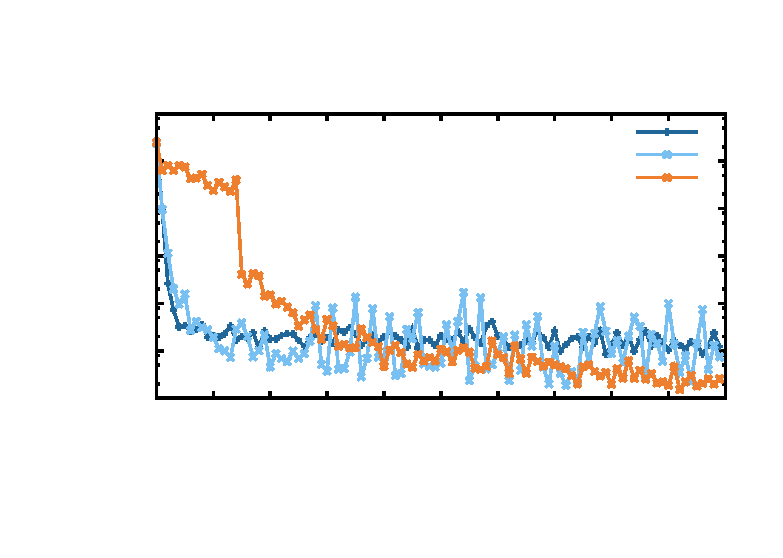
\includegraphics{sin}}%
    \gplfronttext
  \end{picture}%
\endgroup
}
\caption{Sine function approximation by different methods.}
\label{fig:sin_loss}
\end{figure}

It is immediately clear that our method is able to converge to a much better solution than simple training methods.
Importantly, we plot the y-axis on the logarithmic scale, so small improvement are in fact extremely significant.
Firstly, we note that increasing the capacity of the network from 100 to 500 nodes does not have a significant impact on final error.
In fact, the 500-node result would generally be considered worse, as it exhibits far noisier behavior.
To measure these results quantitatively, we consider both the average and the standard deviations of loss over the final 10 samples.
These results are presented in Table~\ref{table:sin_errors}.
We can see that the noisier results of the 500-node network are actually noticeably worse when averaged---it has nearly twice the error of the smaller 100-node network.
Furthermore, the standard deviation is an order of magnitude larger over the 100-node network., which is extremely poor as it is larger than the average error.
In contrast, the adaptive method exhibits both lower mean and standard deviation

\begin{table}[!htb]
\centering
\caption{Final-10 errors for various methods.}
\label{table:sin_errors}
\begin{tabular}{@{}lrr@{}}
\toprule
Network  & Mean    & Standard Deviation \\ \midrule
100-node & 0.00138 & 0.000389           \\
500-node & 0.00234 & 0.003261           \\
Adaptive & 0.00024 & 0.000084           \\ \bottomrule
\end{tabular}
\end{table}



\section{MNIST Classifier}
Modern deep learning algorithms have generally tended to be developed for image classification purposes, in part due to the original usage of convolutional neural networks.
LeCun et al.'s original work with CNNs \cite{lecun1998gradient} was in designing a classifier for the MNIST dataset, a collection of monochrome handwritten digits 

Tensorflow includes MNIST support as part of the base installation

\emph{ < As above, this was in my presentation. Results were good, but not as improved as the previous example. Also, it's important to note that small improvements to MNIST are pretty big because of high accuracy overall (99.32 vs 99.37 accuracy) > }


\section{CIFAR-100}
One of the common modern image classification datasets is CIFAR-100, a set of 60000 images collected by researchers at the University of Toronto.
It consists of 20 classes, each with 5 subclasses.
For each of the 100 subclasses, there are 500 training images and 100 testing images.
The images are in color, but are of low resolution at $32\times 32$; the small size of the dataset makes it especially attractive as an experimental problem; a few sample images are shown in Figure~\ref{fig:cifar100}.
Larger image classification datasets exist, such as the commonly used ImageNet, but due to its over 150GB download size and consequently longer training times, it was not considered for this thesis.
Most modern deep learning papers include results on both CIFAR-10 (a smaller version of the same problem) and CIFAR-100; we choose CIFAR-100 as state of the art performance on CIFAR-10 is over 90\%, leading to a closer and less separable grouping of experimental results.
In doing this, we hope to avoid the problem seen on the MNIST problem, where it is extremely difficult to improve on results that are already nearly perfect.

\begin{figure}[!htb]
\centering
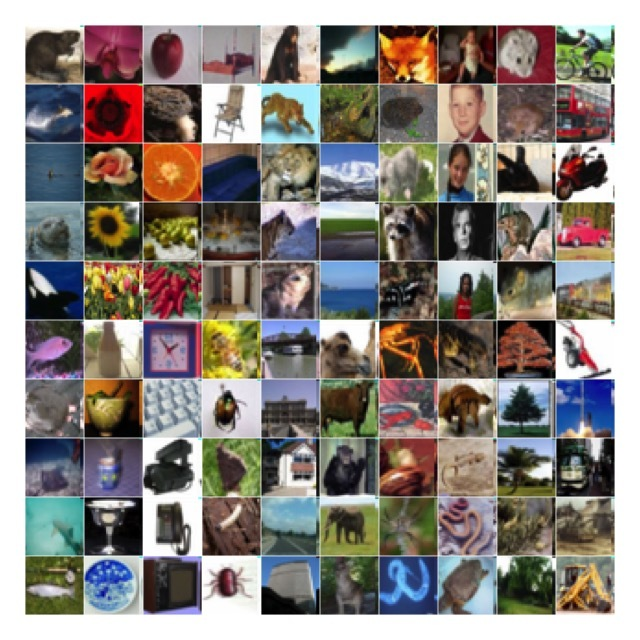
\includegraphics[width=0.5\textwidth]{images/cifar100}
\caption{An example set of images from CIFAR-100. From \cite{cifar100-sample}}
\label{fig:cifar100}
\end{figure}

A particular point of interest with CIFAR-100 is that there are relatively few images per class.
This means that it is a dataset for which overfitting is a critical concern.
Typical algorithms, without any specially designed methods, can often achieve around 60\% accuracy on the testing dataset.
This, however, tends to represent a hard limit, as training accuracy will usually hit nearly 100\% accuracy, meaning that the network has learned all it can from the training dataset.
The difference between testing and training accuracy, especially with the limited data available, is the primary area of improvement for modern algorithms.

We perform a base experiment on a residual network with 30 residual blocks (60 layers), with channel sizes starting at 16 and increasing by a factor of two every 10 layers.
This structure is an adapation of the original residual network, which was built for the ImageNet dataset, to CIFAR-100, which has much smaller images and therefore requires less capacity in the network.
Again utilizing common practice, we use minibatches of size 128, and sample training accuracy every 100 steps.
We allow training to proceed until error rates drop inperceptibly over a reasonably significant period of time; while this requires human judgment, it was also performed due to general time constraints.
We see the expected training accuracy go to 100\%, but the testing accuracy hovers around 65\%, which is also in line with expectations.

In our first experiment, we again use the same basic algorithm first developed for the sine experiment and let the network learn in tenths.
Observing the error rates from the static experiment, we let the network expand every 25 samples (representing 2500 steps).
This is an extremely restrictive network, and our results show that this is perhaps overconstrained for the problem; the training error peaks at 80\% while the testing error hovers around 58\%.
While this is a noticeably poorer result, it is still interesting to note that the generalization appears to be better in this experiment, as the difference between the training and testing error falls from 35\% to 22\%.
Even in the prior static baseline, there was never a comparably small difference between the training and testing error.
This leads us to consider what might be the beginnings of a generalizability metric, which we discuss in the following chapter.

We also note that that accuracy on the dataset is just one measure of precision.
During our experiments, we also log the cross-entropy loss, which provides a sense of not just how likely the network was to get the right answer, but how confidently it did so.
That is, while the accuracy is determined by picking the category with the highest activation, it may have been a very close 
For example, on a binary classification problem with classes 0 and 1, where the correct response is nearly always 1, a network with constant output activations $[0.49, 0.51]$ would have extremely low error but high cross-entropy loss.
Using this metric, we note that the cross-entropy loss is lower at the same training error for our methodology, indicating that its outputs are more regularized.

These results are summarized in table


\section{Performance}
We note that our algorithm involves nearly no overhead over the original architecture; a simple timing benchmark over 1000 epochs of MNIST indicates a performance difference of 3.5\% (37.9 seconds versus 36.6 seconds), which is well within the margin of error.
Furthermore, by limiting the capacity of the network, we are able to achieve far faster initial training.
The initial timing experiment was performed by applying the algorithm but forcing it to use the full capacity of the network initially; this is far from the original intent.
By utilizing it in the same way as developed for the experiments, the first 1000 epochs of MNIST actually take 11.9 seconds, which is a huge improvement.
This performance boost can make a significant difference over the course of a training cycle.
While the algorithm takes more epochs to converge, the increased speed of working through the initial epochs is a significant boon.
In general, any decrease in performance can likely be attributed to the more intricate methods required to perform basic variable operations, recalling Listing~\ref{lst:var_deconst}.
These are generally considered to be minor; in fact, for most researchers, the choice of deep learning library is rarely for performance reasons, especially for single-GPU servers.
Nearly all of the time spent is within the intricacies of the CUDNN module which interfaces directly with the GPU.
Our algorithm adds effectively no stress to the GPU, and even when running at full capacity can speed up training by fixing portions of the network, thus eliminating the need to perform the expensive gradient calculations.

\emph{ < Expanding on performance gains here because of the smaller trained network. Also, Tensorflow imposes some other interesting details here because of the array slicing necessary. > }
